\section{Consuntivo}
In questa sezione del documento viene riportata la distribuzione reale delle risorse del gruppo nei vari periodi dello sviluppo del progetto, confrontandole con quelle preventivate.\\
Il bilancio potrà essere:
\begin{itemize}
	\item \textbf{Positivo} se il costo totale del periodo analizzato è minore di quello preventivato;
	\item \textbf{In pari} se il costo totale del periodo analizzato è uguale a quello preventivato;
	\item \textbf{Negativo} se il costo totale del periodo analizzato è superiore di quello preventivato.
\end{itemize}

\subsection{Analisi}
%
% ----------------------------------------------------------------------------------------------------------------
\subsubsection{Consuntivo sprint\textsubscript{G} I}

Questa tabella mostra come le risorse del gruppo sono state utilizzate realmente nel primo sprint\textsubscript{G} del progetto, svolto nel periodo di analisi, e le confronta con quelle preventivate.
% ----------------------------------------------------------------------------------------------------------------

\setlength\extrarowheight{5pt}
\rowcolors{2}{gray!10}{gray!40}
\begin{tabularx}{\textwidth}{|c|XcXX|c|}
	\hline
	\rowcolor{white}
	\textbf{Ruolo} & \textbf{Ore preventivate} & \textbf{Ore reali} & \textbf{Costo preventivato (€)} & \textbf{Costo reale (€)} & \textbf{Errore (€)} \\
	\hline
	Responsabile &6&6&180&180&+0\\
	Amministratore &26&28 (+2)&520&560&+40\\
	Analista &28&26 (-2)&700&650&-50\\
	Verificatore &-&-&-&-&-\\
	Programmatore &-&-&-&-&-\\
	Progettista &-&-&-&-&- \\
	\hline
	Totale &60&60&1400&1390&-10\\
	\hline
	\rowcolor{white}
	\caption{Consuntivo ore e costi per ruolo del primo sprint\textsubscript{G}}
\end{tabularx}
\subsubsection{Analisi retrospettiva sprint\textsubscript{G} I}
Nello sprint\textsubscript{G} I le ore preventivate per ogni ruolo sono state piuttosto accurate rispetto a quelle reali, tenendo conto che il gruppo ha scelto di dedicare delle ore in più al ruolo di amministratore e meno a quello dell'analista per poter definire fin da subito delle basi per il way of working e per avere una buona comprensione dell'ambiente di lavoro scelto. Avendo sottratto delle ore dal ruolo dell'analista, che è stato meno necessario di quanto preventivato in questo primo sprint\textsubscript{G}, il gruppo è riuscito a non sforare i costi preventivati.


% ----------------------------------------------------------------------------------------------------------------

\newpage
\subsubsection{Consuntivo sprint\textsubscript{G} II}
Questa tabella mostra come le risorse del gruppo sono state utilizzate realmente nel secondo sprint\textsubscript{G} del progetto, svolto nel periodo di analisi, e le confronta con quelle preventivate.
% ----------------------------------------------------------------------------------------------------------------

\setlength\extrarowheight{5pt}
\rowcolors{2}{gray!10}{gray!40}
\begin{tabularx}{\textwidth}{|c|XcXX|c|}
	\hline
	\rowcolor{white}
	\textbf{Ruolo} & \textbf{Ore preventivate} & \textbf{Ore reali} & \textbf{Costo preventivato (€)} & \textbf{Costo reale (€)} & \textbf{Errore (€)} \\
	\hline
	Responsabile &6&8 (+2)&180&240&+60\\
	Amministratore &16&16&320&320&+0\\
	Analista &41&44 (+3)&1025&1100&+75\\
	Verificatore &27&25 (-2)&405&375&-30\\
	Programmatore &-&-&-&-&-\\
	Progettista &-&-&-&-&-\\
	\hline
	Totale &90&93 (+3)&1930&2035&+105\\
	\hline
	\rowcolor{white}
	\caption{Consuntivo ore e costi per ruolo del secondo sprint\textsubscript{G}}
\end{tabularx}
\subsubsection{Analisi retrospettiva sprint\textsubscript{G} II}
Nello sprint\textsubscript{G} II si è reso necessario utilizzare ore in più per il ruolo di analista a causa di alcune difficoltà riscontrate nello svolgimento dell'attività di analisi dei requisiti\textsubscript{G}, dovute soprattutto all'inesperienza del gruppo in questo campo. Attraverso alcuni incontri con il proponente e con il professor Cardin, il gruppo pur utilizzando più ore del previsto è riuscita a risolvere i dubbi riscontrati e procedere. Le ore aggiuntive del responsabile sono state utilizzate per l'attività di pianificazione del progetto e delle sue attività, in modo che lo svolgimento di questo potesse essere il più efficiente ed efficace possibile. 

% ----------------------------------------------------------------------------------------------------------------
\newpage
\subsubsection{Consuntivo sprint\textsubscript{G} III}
Questa tabella mostra come le risorse del gruppo sono state utilizzate realmente nel terzo sprint\textsubscript{G} del progetto, svolto nel periodo di analisi, e le confronta con quelle preventivate.
% ----------------------------------------------------------------------------------------------------------------

\setlength\extrarowheight{5pt}
\rowcolors{2}{gray!10}{gray!40}
\begin{tabularx}{\textwidth}{|c|XcXX|c|}
	\hline
	\rowcolor{white}
	\textbf{Ruolo} & \textbf{Ore preventivate} & \textbf{Ore reali} & \textbf{Costo preventivato (€)} & \textbf{Costo reale (€)} & \textbf{Errore (€)} \\
	\hline
	Responsabile &3&3&90&90&+0\\
	Amministratore &6&7 (+1)&120&140&+20\\
	Analista &8&6 (-2)&200&150&-50\\
	Verificatore &13&15 (+2)&195&225&+30\\
	Programmatore &-&-&-&-&-\\
	Progettista &-&-&-&-&- \\
	\hline
	Totale &30&31 (+1)&605&605&+0\\
	\hline
	\rowcolor{white}
	\caption{Consuntivo ore e costi per ruolo del terzo sprint\textsubscript{G}}
\end{tabularx}
\subsubsection{Analisi retrospettiva sprint\textsubscript{G} III}
Nello sprint\textsubscript{G} III si è scelto di dare più importanza al ruolo del verificatore, fondamentale per consolidare quanto fatto fino a quel momento. Considerando che lo sforamento delle ore preventivate all'analista nello sprint\textsubscript{G} precedente ha permesso di avere delle basi solide di analisi dei requisiti\textsubscript{G} già all'inizio di questo sprint\textsubscript{G}, il ruolo di analista ha necessitato di meno ore di quelle preventivate. Nel complesso non ci sono stati aumenti dei costi per questo sprint\textsubscript{G}.

% ----------------------------------------------------------------------------------------------------------------
\newpage
\subsubsection{Consuntivo sprint\textsubscript{G} V}
Questa tabella mostra come le risorse del gruppo sono state utilizzate realmente nel quinto sprint\textsubscript{G} del progetto, svolto nel periodo di analisi in parallelo al periodo di produzione del proof of concept, e le confronta con quelle preventivate.
% ----------------------------------------------------------------------------------------------------------------

\setlength\extrarowheight{5pt}
\rowcolors{2}{gray!10}{gray!40}
\begin{tabularx}{\textwidth}{|c|XcXX|c|}
	\hline
	\rowcolor{white}
	\textbf{Ruolo} & \textbf{Ore preventivate} & \textbf{Ore reali} & \textbf{Costo preventivato (€)} & \textbf{Costo reale (€)} & \textbf{Errore (€)} \\
	\hline
	Responsabile &3&4 (+1)&90&120&+30\\
	Amministratore &3& 3&60&60&+0\\
	Analista &5&4 (-1)&125&100&-25\\
	Verificatore &7&8 (+1)&105&120&+15\\
	Programmatore &-&-&-&-&-\\
	Progettista &-&-&-&-&- \\
	\hline
	Totale &18&19 (+1)&380&400&+20\\
	\hline
	\rowcolor{white}
	\caption{Consuntivo ore e costi per ruolo del quinto sprint\textsubscript{G}}
\end{tabularx}
\subsubsection{Analisi retrospettiva sprint\textsubscript{G} V}
Nello sprint\textsubscript{G} V le ore preventivate per ogni ruolo sono state piuttosto accurate rispetto a quelle reali, con delle differenze minime che hanno portato ad un aumento dei costi poco significativo. Le modifiche ai requisiti\textsubscript{G}, ottenute dal riscontro con i risultati del PoC\textsubscript{G}, sono state meno significative di quanto preventivato. Hanno richiesto invece del tempo in più le attività di verifica\textsubscript{G} dei vari documenti redatti.

% ----------------------------------------------------------------------------------------------------------------
\newpage
\subsubsection{Consuntivo sprint\textsubscript{G} VI}
Questa tabella mostra come le risorse del gruppo sono state utilizzate realmente nel sesto sprint\textsubscript{G} del progetto, svolto nel periodo di analisi e le confronta con quelle preventivate.
% ----------------------------------------------------------------------------------------------------------------

\setlength\extrarowheight{5pt}
\rowcolors{2}{gray!10}{gray!40}
\begin{tabularx}{\textwidth}{|c|XcXX|c|}
	\hline
	\rowcolor{white}
	\textbf{Ruolo} & \textbf{Ore preventivate} & \textbf{Ore reali} & \textbf{Costo preventivato (€)} & \textbf{Costo reale (€)} & \textbf{Errore (€)} \\
	\hline
	Responsabile &2&4 (+2)&60&120&+60\\
	Amministratore &4&3 (-1)&80&60&-20\\
	Analista &-&1 (+1)&0&25&+25\\
	Verificatore &14&14&210&210&+0\\
	Programmatore &-&-&-&-&-\\
	Progettista &-&-&-&-&- \\
	\hline
	Totale &20&21 (+1)&350&415&+65\\
	\hline
	\rowcolor{white}
	\caption{Consuntivo ore e costi per ruolo del sesto sprint\textsubscript{G}}
\end{tabularx}
\subsubsection{Analisi retrospettiva sprint\textsubscript{G} VI}
Nello sprint\textsubscript{G} VI la differenza più significativa tra le ore preventivate e quelle reali è quella evidenziata nel ruolo del responsabile, che ha dovuto compiere alcuni cambiamenti nella pianificazione, dovuta a dei ritardi causati dall'aver sottovalutato gli impegni esterni al progetto e del conseguente rallentamento dello sviluppo di esso. Il responsabile ha dovuto inoltre gestire la divisione dei vari compiti finalizzati a preparare il materiale necessario per la candidatura alla revisione RTB vista l'imminente scadenza. Ciò ha comportato un aumento dei costi rispetto al preventivo.

% ----------------------------------------------------------------------------------------------------------------
\newpage
\subsubsection{Consuntivo periodo di analisi}
Questa tabella mostra come le risorse del gruppo sono state utilizzate realmente nel periodo di analisi e le confronta con quelle preventivate.
% ----------------------------------------------------------------------------------------------------------------

\setlength\extrarowheight{5pt}
\rowcolors{2}{gray!10}{gray!40}
\begin{tabularx}{\textwidth}{|c|XcXX|c|}
	\hline
	\rowcolor{white}
	\textbf{Ruolo} & \textbf{Ore preventivate} & \textbf{Ore reali} & \textbf{Costo preventivato (€)} & \textbf{Costo reale (€)} & \textbf{Errore (€)} \\
	\hline
	Responsabile &20&25 (+5)&600&750&+150\\
	Amministratore &55&57 (+2)&1100&1140&+40\\
	Analista &82&81 (-1)&2050&2025&-25\\
	Verificatore &61&62 (+1)&915&930&+15\\
	Programmatore &-&-&-&-&-\\
	Progettista &-&-&-&-&-\\
	\hline
	Totale &218&225 (+7)&4665&4845&+180\\
	\hline
	\rowcolor{white}
	\caption{Consuntivo ore e costi per ruolo durante il periodo di analisi}
\end{tabularx}

\subsubsection{Conclusioni per il periodo di analisi}
Valutando con occhio critico il consuntivo del periodo di analisi, gli errori più significativi sono stati i seguenti:
\begin{itemize}
	\item Il ruolo di responsabile ha richiesto ore aggiuntive per poter monitorare l'avanzamento delle attività e la pianificazione di esse, viste le dimensioni del progetto e la poca esperienza dei membri del gruppo nella gestione di progetto;
    \item Il ruolo di amministratore ha richiesto ore aggiuntive per poter definire un way of working che potesse essere una solida base allo sviluppo futuro e che riuscisse a far collaborare efficacemente tutti i membri del gruppo.
\end{itemize}
Un punto critico di questo periodo è stato il sottovalutare alcuni rischi riscontrati. Per questo motivo il gruppo si impegnerà a mitigare meglio i rischi analizzati.
% ----------------------------------------------------------------------------------------------------------------
\newpage
\subsection{Produzione del proof of concept}
%
% ----------------------------------------------------------------------------------------------------------------
\subsubsection{Consuntivo sprint\textsubscript{G} IV}

Questa tabella mostra come le risorse del gruppo sono state utilizzate realmente nel quarto sprint\textsubscript{G} del progetto, svolto nel periodo di produzione del proof of concept, e le confronta con quelle preventivate.
% ----------------------------------------------------------------------------------------------------------------

\setlength\extrarowheight{5pt}
\rowcolors{2}{gray!10}{gray!40}
\begin{tabularx}{\textwidth}{|c|XcXX|c|}
	\hline
	\rowcolor{white}
	\textbf{Ruolo} & \textbf{Ore preventivate} & \textbf{Ore reali} & \textbf{Costo preventivato (€)} & \textbf{Costo reale (€)} & \textbf{Errore (€)} \\
	\hline
	Responsabile &3&2 (-1)&90&60&-30\\
	Amministratore &2&2 &40&40&+0\\
	Analista &2&2&50&50&+0\\
	Verificatore &2&2&30&30&+0\\
	Programmatore &2&4 (+2)&30&60&+30\\
	Progettista &7&6 (-1)&175&150&-25 \\
	\hline
	Totale &18&18&415&390&-25\\
	\hline
	\rowcolor{white}
	\caption{Consuntivo ore e costi per ruolo del quarto sprint\textsubscript{G}}
\end{tabularx}
\subsubsection{Analisi retrospettiva sprint\textsubscript{G} IV}
Nello sprint\textsubscript{G} IV non sono state evidenziate differenze significative tra le ore prevenivate e quelle reali. Al contrario si il gruppo è riuscito a definire più chiaramente del previsto in che direzione si dovesse sviluppare il PoC\textsubscript{G} necessitando di conseguenza di meno ore per i ruoli di responsabile e progettista, riuscendo così a risparmiare sui costi totali.

% ----------------------------------------------------------------------------------------------------------------

\newpage
\subsubsection{Consuntivo sprint\textsubscript{G} V}
Questa tabella mostra come le risorse del gruppo sono state utilizzate realmente nel quinto sprint\textsubscript{G} del progetto, svolto nel periodo di produzione del proof of concept in parallelo al periodo di analisi, e le confronta con quelle preventivate.
% ----------------------------------------------------------------------------------------------------------------

\setlength\extrarowheight{5pt}
\rowcolors{2}{gray!10}{gray!40}
\begin{tabularx}{\textwidth}{|c|XcXX|c|}
	\hline
	\rowcolor{white}
	\textbf{Ruolo} & \textbf{Ore preventivate} & \textbf{Ore reali} & \textbf{Costo preventivato (€)} & \textbf{Costo reale (€)} & \textbf{Errore (€)} \\
	\hline
	Responsabile &3&3&90&90&+0\\
	Amministratore &3&2 (-1)&60&40&-20\\
	Analista &2&2&50&50&+0\\
	Verificatore &7&8 (+1)&105&120&+15\\
	Programmatore &13&16 (+3)&195&240&+45\\
	Progettista &8&6 (-2)&200&150&-50 \\
	\hline
	Totale &36&37 (+1)&700&690&-10\\
	\hline
	\rowcolor{white}
	\caption{Consuntivo ore e costi per ruolo del quinto sprint\textsubscript{G}}
\end{tabularx}
\subsubsection{Analisi retrospettiva sprint\textsubscript{G} V}
Nello sprint\textsubscript{G} V sono state necessarie più ore di programmatore rispetto a quelle preventivate in quanto durante lo sviluppo del PoC\textsubscript{G} alcuni membri del team hanno riscontrato difficoltà nel portare a termine le attività di codifica assegnate, data la poca esperienza con alcune delle tecnologie scelte. Essendo però riusciti a diminuire le ore di amministratore e progettista, le quali sono state meno necessarie di quanto preventivato, a fine sprint\textsubscript{G} non si è verificato un aumento dei costi totali.
% ----------------------------------------------------------------------------------------------------------------
\newpage
\subsubsection{Consuntivo periodo di produzione del proof of concept}
Questa tabella mostra come le risorse del gruppo sono state utilizzate realmente nel periodo di produzione del proof of concept e le confronta con quelle preventivate.
% ----------------------------------------------------------------------------------------------------------------

\setlength\extrarowheight{5pt}
\rowcolors{2}{gray!10}{gray!40}
\begin{tabularx}{\textwidth}{|c|XcXX|c|}
	\hline
	\rowcolor{white}
	\textbf{Ruolo} & \textbf{Ore preventivate} & \textbf{Ore reali} & \textbf{Costo preventivato (€)} & \textbf{Costo reale (€)} & \textbf{Errore (€)} \\
	\hline
	Responsabile &6&5 (-1)&180&150&-30\\
	Amministratore &5&4 (-1)&100&80&-20\\
	Analista &4&4&100&100&+0\\
	Verificatore &9&10 (+1)&135&150&+15\\
	Programmatore &15&20 (+5)&225&300&+75\\
	Progettista &15&12 (-3)&375&300&-75\\
	\hline
	Totale &54&55 (+1)&1115&1080&-35\\
	\hline
	\rowcolor{white}
	\caption{Consuntivo ore e costi per ruolo durante il periodo di produzione del proof of concept}
\end{tabularx}

\subsubsection{Conclusioni per il periodo di produzione del proof of concept}


Valutando con occhio critico il consuntivo del periodo di produzione del proof of concept, gli errori più significativi sono stati i seguenti:
\begin{itemize}
	\item Il ruolo di programmatore ha richiesto ore aggiuntive per poter portare a termine la codifica del PoC\textsubscript{G}, e sono state utilizzate per colmare le lacune tecnologiche dei membri del gruppo;
    \item Il ruolo di progettista ha richiesto meno ore rispetto a quelle preventivate dal momento che la scelta delle tecnologie  da includere nella realizzazione del PoC\textsubscript{G} ha richiesto meno tempo del previsto.
\end{itemize}
Il gruppo è pertanto riuscito a compensare una parte dei costi che hanno superato il preventivo durante il periodo di analisi.

% ----------------------------------------------------------------------------------------------------------------
\newpage
\subsection{Progettazione architetturale}
%
% ----------------------------------------------------------------------------------------------------------------
\subsubsection{Consuntivo sprint\textsubscript{G} VII}

Questa tabella mostra come le risorse del gruppo sono state utilizzate realmente nel settimo sprint\textsubscript{G} del progetto, svolto nel periodo di progettazione architetturale, e le confronta con quelle preventivate.
% ----------------------------------------------------------------------------------------------------------------

\setlength\extrarowheight{5pt}
\rowcolors{2}{gray!10}{gray!40}
\begin{tabularx}{\textwidth}{|c|XcXX|c|}
	\hline
	\rowcolor{white}
	\textbf{Ruolo} & \textbf{Ore preventivate} & \textbf{Ore reali} & \textbf{Costo preventivato (€)} & \textbf{Costo reale (€)} & \textbf{Errore (€)} \\
	\hline
	Responsabile & 6 & 8 (+2) & 180 & 240& +60 \\
	Amministratore & 8 & 6 (-2) & 160 & 120 & -40 \\
	Analista & 3 & 1 (-2) & 75 & 25 & -50 \\
	Verificatore & 10 & 7 (-3) & 150 & 105 & -45 \\
	Programmatore & - & - & - & - & - \\
	Progettista & 39 & 45 (+6) & 975 & 1125 & +150 \\
	\hline
	Totale & 66 & 67 (+1) & 1540 & 1615 & +75 \\
	\hline
	\rowcolor{white}
	\caption{Consuntivo ore e costi per ruolo del settimo sprint\textsubscript{G}}
\end{tabularx}
\subsubsection{Analisi retrospettiva sprint\textsubscript{G} VII}

Durante lo sprint\textsubscript{G} VII, è emersa la necessità di dedicare un numero significativamente maggiore di ore al ruolo di progettista rispetto a quanto inizialmente previsto. Durante la fase di progettazione dell'architettura del progetto, i membri del gruppo hanno affrontato difficoltà nella realizzazione del diagramma delle classi, dovuta anche all'inesperienza in questo ambito. Nonostante a ciò il team è riuscito a non sforare di troppo i costi preventivati, riducendo il numero di ore assegnate ad altri ruoli, i quali si sono rivelati meno necessari in questo periodo di progetto. \\
Durante questo sprint\textsubscript{G} il gruppo ha dovuto anche affrontare un secondo problema. Alcuni membri hanno avuto cambiamenti significativi a lungo termine negli impegni settimanali, causando quindi una diminuzione nelle ore che potevano dedicare al progetto. Questo ha reso necessario rivedere la distribuzione delle ore per i vari membri, per non avere un carico di lavoro sbilanciato ma soprattutto di cambiare le scadenze fissate precedentemente, che dovevano essere ricalcolate in base al nuovo numero di ore produttive che il gruppo poteva fornire settimanalmente. Questa attività ha richiesto alcune settimane e sono state necessarie delle ore in più per il ruolo di responsabile, dato che si è prima dovuto comprendere a pieno come sarebbe cambiato lo sviluppo del progetto a seguito del cambiamento. 

\subsubsection{Conclusioni per il periodo di progettazione architetturale}

Valutando con occhio critico il consuntivo del periodo di progettazione architetturale, gli errori più significativi sono stati i seguenti:
\begin{itemize}
	\item Il ruolo di progettista ha richiesto ore aggiuntive per completare il diagramma delle classi, più precisamente sono state organizzate degli incontri a fine settimana dedicati alla discussione e alla realizzazione del diagramma;
	\item Il ruolo di responsabile ha avuto necessità di ore in più per rivedere la distribuzione delle ore e scadenze del progetto;
	\item Gli altri ruoli hanno richiesto meno ore poiché le attività associate a tali ruoli non erano numerose o complesse come nel caso del ruolo di progettista.
\end{itemize}
L'utilizzo di ore in più e il leggero sforo nei costi durante questo sprint\textsubscript{G} è stato anche un investimento per la gestione del progetto futura.


% ----------------------------------------------------------------------------------------------------------------
\newpage
\subsection{Progettazione di dettaglio e codifica}
%
% ----------------------------------------------------------------------------------------------------------------
\subsubsection{Consuntivo sprint\textsubscript{G} VIII}

Questa tabella mostra come le risorse del gruppo sono state utilizzate realmente nel ottavo sprint\textsubscript{G} del progetto, svolto nel primo periodo di progettazione di dettaglio e codifica, e le confronta con quelle preventivate.
% ----------------------------------------------------------------------------------------------------------------

\setlength\extrarowheight{5pt}
\rowcolors{2}{gray!10}{gray!40}
\begin{tabularx}{\textwidth}{|c|XcXX|c|}
	\hline
	\rowcolor{white}
	\textbf{Ruolo} & \textbf{Ore preventivate} & \textbf{Ore reali} & \textbf{Costo preventivato (€)} & \textbf{Costo reale (€)} & \textbf{Errore (€)} \\
	\hline
	Responsabile & 3 & 3 & 90 & 90 & 0 \\
	Amministratore & 3 & 2 (-1) & 60 & 40 & -20 \\
	Analista & - & - & - & - & - \\
	Verificatore & 5 & 6 (+1) & 75 & 90 & +15 \\
	Programmatore & 6 & 18 (+12) & 90 & 270 & +180 \\
	Progettista & 19 & 	14 (-5) & 475 & 350 & -125 \\
	\hline
	Totale & 36 & 43 (+7) & 790 & 840 & +50 \\
	\hline
	\rowcolor{white}
	\caption{Consuntivo ore e costi per ruolo del ottavo sprint\textsubscript{G}}
\end{tabularx}
\subsubsection{Analisi retrospettiva sprint\textsubscript{G} VIII}

Durante lo sprint\textsubscript{G} VIII, si è riscontrato un significativo aumento delle ore dedicate al ruolo di programmatore. 
Durante la fase di progettazione architetturale, è emersa la necessità di adottare il framework\textsubscript{G} Laravel, a seguito anche dell'analisi fatta durante l'incontro per la technology baseline con il professor Cardin. Di conseguenza, i membri del team hanno dovuto dedicare ore extra per acquisire le competenze necessarie nell'utilizzo di questo framework\textsubscript{G}.
Date però le buone fondamenta di progettazione architetturale, dovute anche alle ore in più utilizzate dal gruppo nello sprint\textsubscript{G} VII, la progettazione di dettaglio si è svolta senza imprevisti ed ha utilizzato meno ore di quelle preventivate.
In questo sprint\textsubscript{G} si sono dovute utilizzare più ore di quelle programmate, anche per un errore commesso durante il periodo di analisi, nella quale non si era pensato necessario l'utilizzo di un framework.

% ----------------------------------------------------------------------------------------------------------------
\newpage
\subsubsection{Consuntivo sprint\textsubscript{G} IX}

Questa tabella mostra come le risorse del gruppo sono state utilizzate realmente nel nono sprint\textsubscript{G} del progetto, svolto nel secondo periodo di progettazione di dettaglio e codifica, e le confronta con quelle preventivate.
% ----------------------------------------------------------------------------------------------------------------

\setlength\extrarowheight{5pt}
\rowcolors{2}{gray!10}{gray!40}
\begin{tabularx}{\textwidth}{|c|XcXX|c|}
	\hline
	\rowcolor{white}
	\textbf{Ruolo} & \textbf{Ore preventivate} & \textbf{Ore reali} & \textbf{Costo preventivato (€)} & \textbf{Costo reale (€)} & \textbf{Errore (€)} \\
	\hline
	Responsabile & 2 & 2 & 60 & 60 & 0 \\
	Amministratore & 5 & 5 & 100 & 100 & 0 \\
	Analista & - & - & - & - & - \\
	Verificatore & 10 & 10 (+2) & 150 & 180 & +30 \\
	Programmatore & 50 & 45 (-5) & 750 & 675 (-75) & -75 \\
	Progettista & 3 & 2 (-1) & 75 & 50 (-25) & -25 \\
	\hline
	Totale & 70 & 66 (-4) & 1135 & 1065 & -70 \\
	\hline
	\rowcolor{white}
	\caption{Consuntivo ore e costi per ruolo del nono sprint\textsubscript{G}}
\end{tabularx}
\subsubsection{Analisi retrospettiva sprint\textsubscript{G} IX}

Nello sprint\textsubscript{G} IX, il team è riuscito a completare in le attività di codifica relative ai requisiti obbligatori utilizzando meno ore di quelle preventivate. Questo grazie all'utilizzo del framework\textsubscript{G} Laravel, che ha permesso di semplificare di molto alcune parti di codifica del prodotto.
Si sono rese necessarie alcune ore in più per il ruolo di verificatore, per l'analisi e i test sul codice.

% ----------------------------------------------------------------------------------------------------------------
\newpage
\subsubsection{Consuntivo sprint\textsubscript{G} X}

Questa tabella mostra come le risorse del gruppo sono state utilizzate realmente nel decimo sprint\textsubscript{G} del progetto, svolto nel terzo periodo di progettazione di dettaglio e codifica, e le confronta con quelle preventivate.
% ----------------------------------------------------------------------------------------------------------------

\setlength\extrarowheight{5pt}
\rowcolors{2}{gray!10}{gray!40}
\begin{tabularx}{\textwidth}{|c|XcXX|c|}
	\hline
	\rowcolor{white}
	\textbf{Ruolo} & \textbf{Ore preventivate} & \textbf{Ore reali} & \textbf{Costo preventivato (€)} & \textbf{Costo reale (€)} & \textbf{Errore (€)} \\
	\hline
	Responsabile & 1 & 2 (+1) & 30 & 60 & +30 \\
	Amministratore & 1 & 2 (+1) & 20 & 20 & +20 \\
	Analista & - & - & - & - & - \\
	Verificatore & 6 & 8 (+2) & 90 & 120 & +30 \\
	Programmatore & 21 & 18 (-3) & 315 & 270 & -40 \\
	Progettista & 1 & 1 & 25 & 25 & 0 \\
	\hline
	Totale & 30 & 31 (+1) & 480 & 520 & +40 \\
	\hline
	\rowcolor{white}
	\caption{Consuntivo ore e costi per ruolo del decimo sprint\textsubscript{G}}
\end{tabularx}

\subsubsection{Analisi retrospettiva sprint\textsubscript{G} X}

Nello sprint\textsubscript{G} X non sono state evidenziate differenze significative rispetto alle ore preventivate. Al contrario il team è riuscito a terminare le attività di codifica utilizzando meno ore del previsto. I ruoli di responsabile e amministratore si sono occupati di gestire rispettivamente la suddivisione delle attività per il completamento della codifica e la gestione del server nella quale è presente il servizio API.

% ----------------------------------------------------------------------------------------------------------------
\newpage
\subsubsection{Consuntivo periodo di progettazione di dettaglio e codifica}
Questa tabella mostra come le risorse del gruppo sono state utilizzate realmente nel periodo della progettazione di dettaglio e codifica e le confronta con quelle preventivate.
% ----------------------------------------------------------------------------------------------------------------

\setlength\extrarowheight{5pt}
\rowcolors{2}{gray!10}{gray!40}
\begin{tabularx}{\textwidth}{|c|XcXX|c|}
	\hline
	\rowcolor{white}
	\textbf{Ruolo} & \textbf{Ore preventivate} & \textbf{Ore reali} & \textbf{Costo preventivato (€)} & \textbf{Costo reale (€)} & \textbf{Errore (€)} \\
	\hline
	Responsabile & 6 & 7 (+1) & 180 & 210 & +30 \\
	Amministratore & 9 & 9 & 180 & 180 & 0 \\
	Analista & - & - & - & - & - \\
	Verificatore & 21 & 26 (+5) & 315 & 390 & +75 \\
	Programmatore & 77 & 81 (+4) & 1155 & 1205 & +60 \\
	Progettista & 23 & 17 (-6) & 575 & 425 & -150 \\
	\hline
	Totale & 136 & 140 (+4) & 2405 & 2420 & +15 \\
	\hline
	\rowcolor{white}
	\caption{Consuntivo ore e costi per ruolo durante il periodo di progettazione di dettaglio e codifica}
\end{tabularx}

\subsubsection{Conclusioni per il periodo di progettazione di dettaglio e codifica}

Valutando con occhio critico il consuntivo del periodo di progettazione di dettaglio e codifica il punto critico
più significativo è stato il tempo in più utilizzato per il ruolo di programmatore per apprendere il framework\textsubscript{G}, ma i risultati sono stati positivi e la fatta ha ripagato a posteriori. 
L'uso del framework\textsubscript{G} non solo ha permesso di risparmiare tempo nella codifica nelle fasi successive, ma anche di rendere il codice prodotto più chiaro e strutturato meglio.\\

In generale, le ore effettive non differiscono eccessivamente da quelle previste, sebbene sia stato necessario dedicare un po' più di tempo del previsto.


% ----------------------------------------------------------------------------------------------------------------
\newpage
\subsection{Validazione e collaudo}
%
% ----------------------------------------------------------------------------------------------------------------
\subsubsection{Consuntivo sprint\textsubscript{G} XI}

Questa tabella mostra come le risorse del gruppo sono state utilizzate realmente nel undicesimo sprint\textsubscript{G} del progetto, svolto nel periodo di validazione e collaudo, e le confronta con quelle preventivate.
% ----------------------------------------------------------------------------------------------------------------

\setlength\extrarowheight{5pt}
\rowcolors{2}{gray!10}{gray!40}
\begin{tabularx}{\textwidth}{|c|XcXX|c|}
	\hline
	\rowcolor{white}
	\textbf{Ruolo} & \textbf{Ore preventivate} & \textbf{Ore reali} & \textbf{Costo preventivato (€)} & \textbf{Costo reale (€)} & \textbf{Errore (€)} \\
	\hline
	Responsabile & 11 & 11 & 330 & 330 & 0 \\
	Amministratore & 8 & 6 (-2) & 160 & 120 & -40 \\
	Analista & - & - & - & - & - \\
	Verificatore & 37 & 35 (-2) & 555 & 525 & -30 \\
	Programmatore & 10 & 12 (+2) & 150 & 180 & +30 \\
	Progettista & - & - & - & - & - \\
	\hline
	Totale & 66 & 64 (-2) & 1195 & 1155 & -40 \\
	\hline
	\rowcolor{white}
	\caption{Consuntivo ore e costi per ruolo dell'undicesimo sprint\textsubscript{G}}
\end{tabularx}
\subsubsection{Analisi retrospettiva sprint\textsubscript{G} XI}

Nello sprint\textsubscript{G} X non sono state evidenziate differenze significative rispetto alle ore preventivate.
Le 2 ore di programmatore in più sono state utilizzate per finalizzare il documento di specifica architetturale e ultimare gli ultimi dettagli nel prodotto finale.
Mentre le attività di test e validazione dei documenti hanno impiegato meno tempo di quello preventivato.

\subsubsection{Conclusioni per il periodo di validazione e collaudo}

Valutando attentamente il consuntivo del periodo di validazione e collaudo, il team è riuscito a completare tutte le attività senza superare le ore preventivate. 
Anzi, è stato possibile utilizzare meno ore rispetto a quanto pianificato, date le buone basi presenti dagli sprint\textsubscript{G} precedenti, compensando quindi lo sforo di ore nel periodo precedente.




% ----------------------------------------------------------------------------------------------------------------
\newpage

\subsection{Consuntivo totale di progetto}
Viene di seguito illustrata una comparazione tra il preventivo iniziale del costo di progetto e quello calcolato al termine di esso.
\setlength\extrarowheight{5pt}
\rowcolors{2}{gray!10}{gray!40}
\begin{tabularx}{\textwidth}{|c|XcXX|c|}
	\hline
	\rowcolor{white}
	\textbf{Ruolo} & \textbf{Ore preventivate} & \textbf{Ore reali} & \textbf{Costo preventivato (€)} & \textbf{Costo reale (€)} & \textbf{Errore (€)} \\
	\hline
	Responsabile &49& 56 (+7) &1470&1680& +210 \\ 
	Amministratore &85& 82 (-3) &1700&1640& -60\\
	Analista &89&86 (-3)&2225&2150& -75 \\
	Verificatore &138&140 (+2)&2070&2100& +30 \\
	Programmatore &102&113 (+11)&1530&1695& +165 \\
	Progettista &77&74 (-3)&1925&1850& -75 \\
	\hline
	Totale &540&551&10920&11115&+195\\
	\hline
	\rowcolor{white}
	\caption{Consuntivo totale di ore e costi per ruolo}
\end{tabularx}


Qui invece illustrata la tabella con tutte le ore rendicontate per ogni membro del gruppo, distribuite per i vari ruoli.
\setlength\extrarowheight{5pt}
\rowcolors{2}{gray!10}{gray!40}
\begin{tabularx}{\textwidth}{|ccccccc|c|}
	\hline
	\rowcolor{white}
	\textbf{Nome} & \textbf{Re} & \textbf{Am} & \textbf{An} & \textbf{Ve} & \textbf{Pr}& \textbf{Pt} & \textbf{Ore totali} \\
	\hline
	Nicola Sinicato &11&12&13&22&22&10&90 \\
	Gabriele Da Re &9&21&11&16&18&14&89 \\
	Luca Brugnera &7&17&15&22&24&10&95 \\
	Matteo Stocco &13&10&14&25&22&11&95 \\
	Ana Lazic &9&10&18&23&15&16&91 \\
	Zhen Wei Zheng &7&12&15&31&13&13&91 \\
	\hline
	Ore totali ruolo &56&82&86&140&113&74&551 \\
	\hline
	\rowcolor{white}
	\caption{Ripartizione complessiva delle ore per ruolo e persona}
\end{tabularx}

\begin{figure}[H]
	\centering
	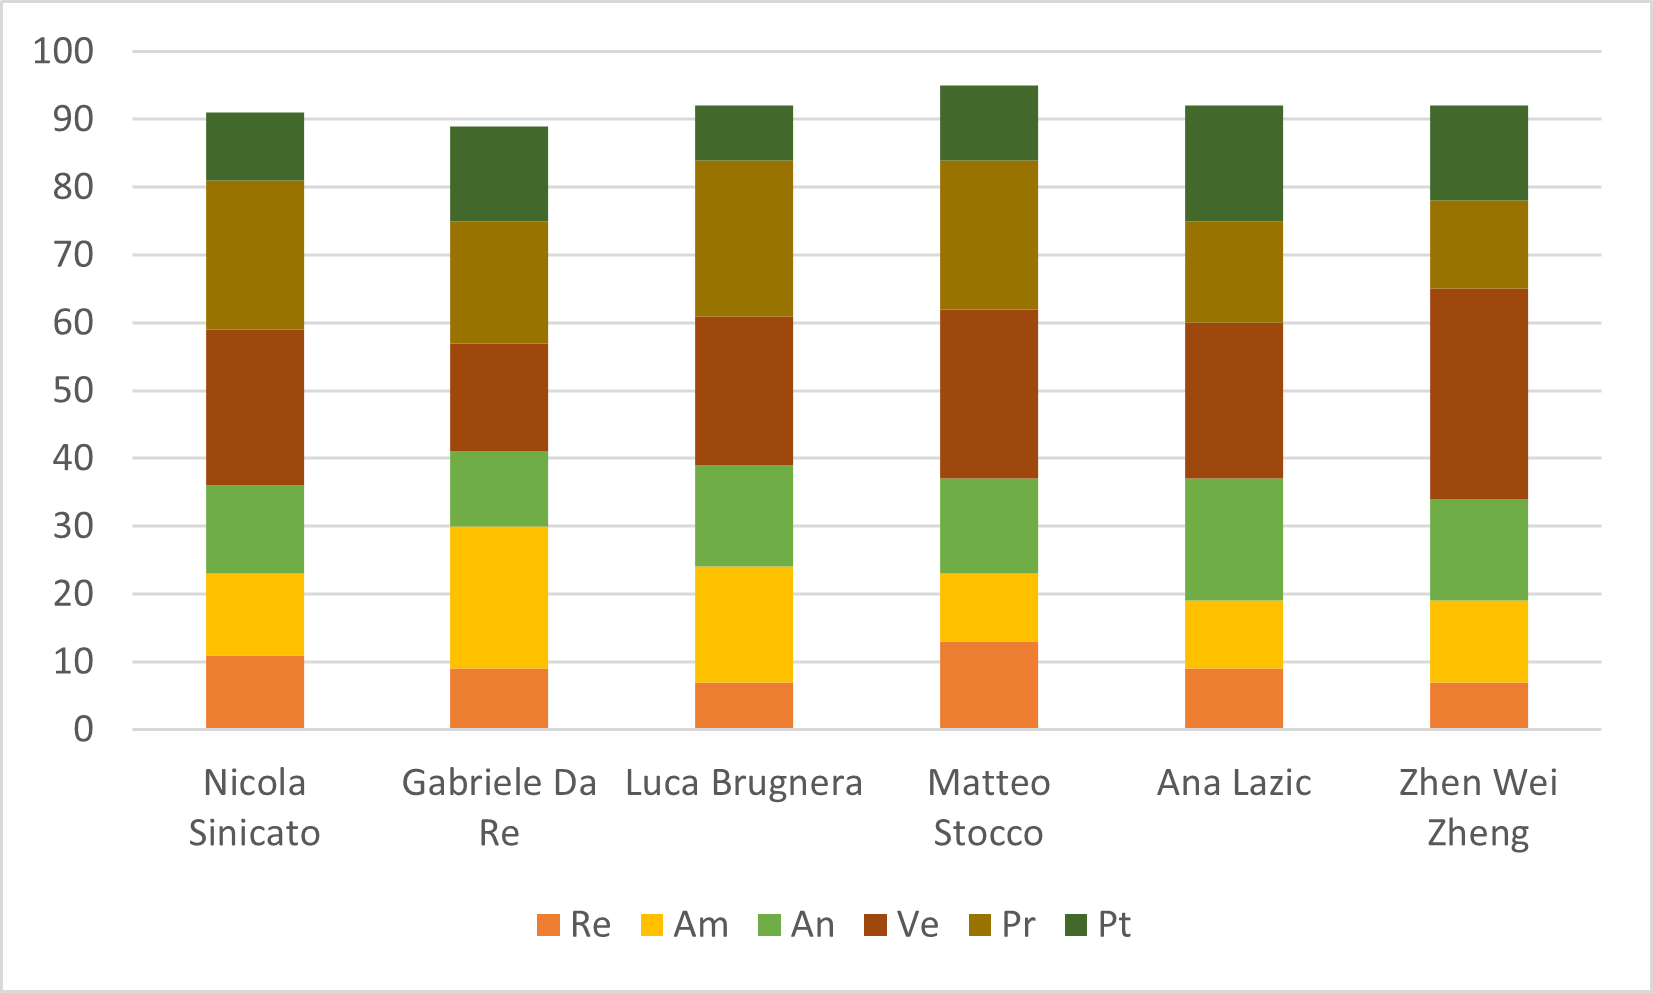
\includegraphics[scale=0.8]{img/consuntivo_membri.png}
	\caption{Istogramma con la distribuzione oraria complessiva}
\end{figure}
\begin{figure}[H]
	\centering
	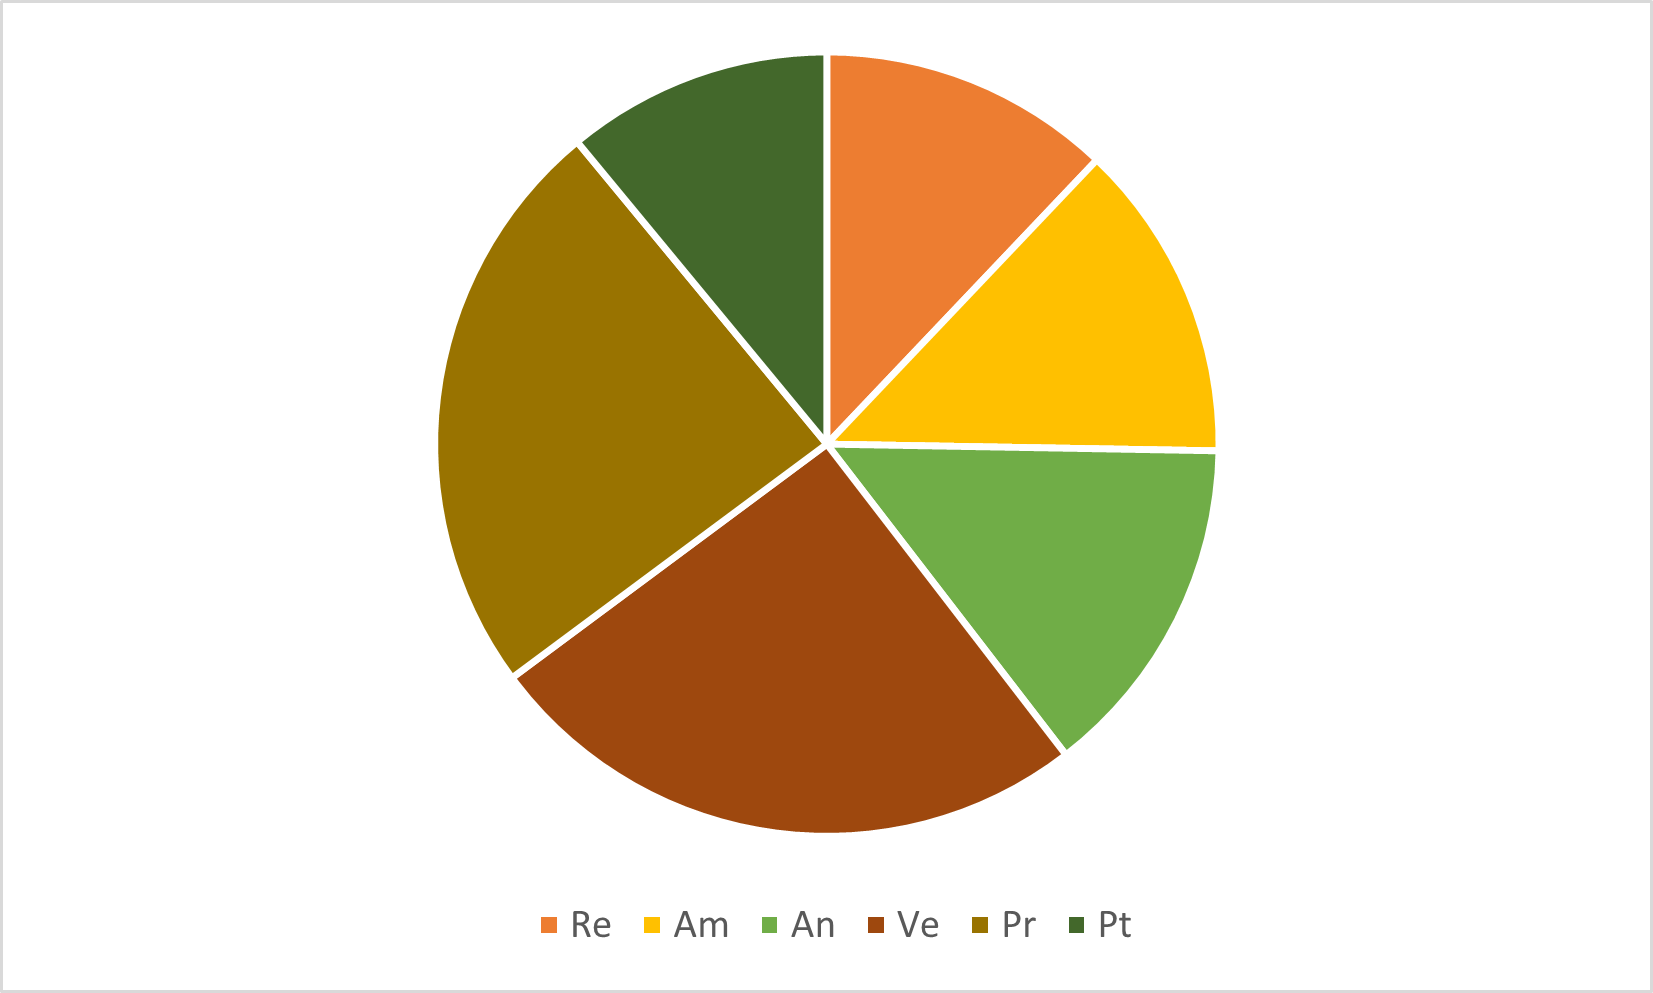
\includegraphics[scale=0.8]{img/consuntivo_ruoli.png}
	\caption{Grafico a torta con la ripartizione delle ore complessive per ruolo}
\end{figure}
